%%%%%%%%%%%%%%%%%%%%%%% file icad-template.tex %%%%%%%%%%%%%%%%%%%%%%%%%
% $Id: icad-template.tex 196 2020-03-20 12:09:24Z foley $
% $URL: https://repository.cs.ru.is/svn/template/tvd/journal/journal-of-physics/icad-template.tex $
% 
% This is a template file for Journal of Physics Conference Series
%   which is used for the International Conference of Axiomatic Design as of 2020
%
%%%%%%%%%%%%%%%%%%%%%%%
\documentclass[a4paper]{jpconf}
\usepackage{graphicx}
\graphicspath{{./}{Graphics/}}

\bibliographystyle{iopart-num}
%\usepackage{citesort}

\usepackage{booktabs}
\usepackage{array} %% needed for advanced table manipulation
%% Column types from http://tex.stackexchange.com/questions/54069/table-with-text-wrapping
\newcolumntype{L}[1]{>{\raggedright\let\newline\\\arraybackslash\hspace{0pt}}m{#1}}
\newcolumntype{C}[1]{>{\centering\let\newline\\\arraybackslash\hspace{0pt}}m{#1}}
\newcolumntype{R}[1]{>{\raggedleft\let\newline\\\arraybackslash\hspace{0pt}}m{#1}}

\usepackage{custom}
\usepackage{url}%%URL should also be the last package loaded along with hyperref if needed


%%%%% Jón 2020-03-20%%%%%%%%%%%%%%%%%%%%%
\usepackage{tikz}
\usetikzlibrary{calc,shadows,shadows.blur}

\def\IosSevenSlider#1#2{
	\tikz[baseline=-0.1cm]{
		\coordinate (start) at (0,0);
		\coordinate (end) at (#1,0);
		\coordinate (mark) at ($(start)!#2!(end)$);
		%\useasboundingbox (start|- 0,-.25) rectangle (end|- 0, .25);
		\draw[line width=0.4mm, line cap=round, blue!50!cyan] 
		(start) -- (mark) edge[lightgray] (end);
		\node[fill=white, draw=lightgray, very thin,
		blur shadow={shadow xshift=0pt, shadow opacity=20, shadow yshift=-0.9mm,
			shadow blur steps=6, shadow blur radius=0.3mm},
		circle, minimum size=0.25cm, inner sep=0pt] at (mark) {};
	}
}
%%%%%%%%%%%%%%%%%%%%%%%%%%%%%%%%%%%%%%%%%%

\begin{document}
\title{Remote Education System}

\author{ J\'on B. Helgason$^{1}$, Hannes A. Magnússon$^{1}$}

\address{$^{1}$Reykjavik University, Menntavegur 1, Reykjavik 102, Iceland}

\ead{jonh16 AT ru.is}

\begin{abstract}
Lightboard needs a lot of expensive and professional equipment and big space for the setup that schools and companies don´t often possess.
By taking a look at lightboard studio and using Axiomatic design method to build a single unit with all the necessary component are present to make it functional lightboard studio.
The solution is a product that is called Lightboard Ready (LR) and is a unit that has a folding mechanism that gives lighting, mic, and camera fixed position and therefore gives an easy user experience.
LR is successful in giving easy user experience, it takes only a few minutes to fold it together and move up to a wall so it won't be in the way when it is not in use. When in need the LR is only a handful of movements away.
\end{abstract}



\section{Introduction}
Teaching STEM field cores effectively need an engaging, personal teaching approach and a lot of feedback. Remote teaching lack every single one of those dimensions and student often struggle with STEM fields when it is taught remotely. Today have lightboard become popular because the teacher faces the camera and can give a lot of eye contact which gives engaging and personal feelings to the course. 
\begin{quote}
	The Lightboard is a glass board, carrying light internally from LED strips along its edges. A video camera captures the presenter and his/her writing by viewing through the glass. The result is vivid, luminous writing floating in front of the presenter, who can now face toward the camera while drawing and interacting with the material on the board.\cite{birdwell2015capturing}
\end{quote}
The problem with lightboards is it needs a lot of expensive professional equipment (lights, cameras, and mic) and an expert to set them up and it needs a lot of space which is not what schools and companies possess often. 
By designing a unit that gives an easy user experience on a lightboard studio it could motivate schools and other companies to use this technology to produce high-quality education material.

\subsection{Customer Needs}\label{CN}
%What would a customer need the item to do?  
%Using Axiomatic Design theory, this is stated as a numbered list of Customer Needs(CN)~\cite{suh1990principles}.
%The top level is \CN0.
%This is often (but not always) decomposed into \CN1, \CN2, etc.
%Here is an example of a top-level:

\begin{quote}
	\textbf{\CN0} : Need to set up lightboard studio easily.
\end{quote}

\begin{quote}
	\textbf{\CN1} : Need to set up camera in correct place.
\end{quote}

\begin{quote} 
	\textbf{\CN2} : Need to set up lights in correct place.
\end{quote}

\begin{quote} 
	\textbf{\CN3} :  Need to set up mic in correct place.
\end{quote}

\begin{quote} 
	\textbf{\CN4} :  Need to take little space when not in use.
\end{quote}

\begin{quote} 
	\textbf{\CN5} :  Need to transport the studio.
\end{quote}

\subsection{Functional Requirements} \label{FR}
The product has to be able to show the material that is being taught to the students
\begin{quote} 
	\textbf{\FR0} : Fold lightboard studio.
\end{quote}

\begin{quote} 
	\textbf{\FR1} :  Guide  the camera to its correct place.
	\\ \textbf{Metric :} Image fills the frame 80-99\%.
\end{quote}

\begin{quote} 
	\textbf{\FR2} :  Guide the lights  to its correct place.
	\\ \textbf{Metric :} Can see face expression.
\end{quote}

\begin{quote} 
	\textbf{\FR3} Guide the mic  to its correct place.
	\\ \textbf{Metric :} Sound is 60-70 db\cite{db}.
\end{quote}

\begin{quote} 
	\textbf{\FR4} :  Fold together.
	\\ \textbf{Metric :} The width is less than 0.8 m.
\end{quote}

\begin{quote} 
	\textbf{\FR5} Move studio in one unit.
	\\ \textbf{Metric :} Can one person move it.
\end{quote}


\begin{figure}[]
	\centering
	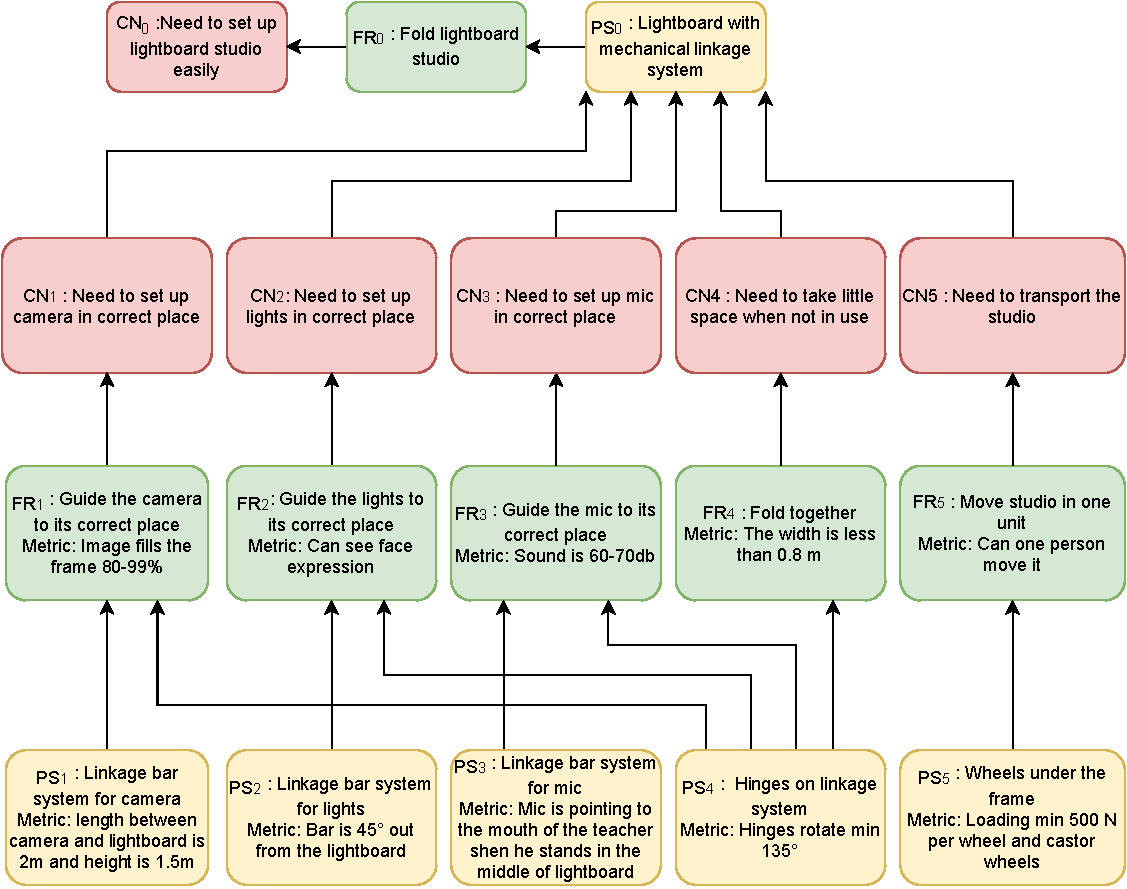
\includegraphics[width=1\textwidth]{matrix.pdf}
	\caption{Design Decomposition flowchart}\label{fig:matrix}
\end{figure}




\section{Background and Prior art}
%Search the internet and books to find out what people are currently doing in this area of research
%How is the problem currently addressed?
% Who and what is trying to solve it, especially the current state of the art? Give company names, product IDs, and specifications
%How do they compare to your general idea (preferably quantitatively)?
%E.g. You can’t say something is cheaper unless you have estimated costs
% Avoid using the word “ good”, “great”,” bad

% Grading sheet 
% History of the problem or product
Today is STEM field remote education done on whiteboards, the problem with them is the teacher turns away from the student or camera when writing and gives a little eye contact. The writing isn't always clear and the teacher is often blocking what he's writing, which gives the class disengaging and impersonal feeling. 
% What similar items (at least 2) exist?
Rocket book has a solution, it called rocket book beacons, its a re-stickable, reusable Beacons convert writing surface into a smartboard by integrating with cloud services in the Rocketbook app.
This product solves only one of the whiteboards problem and that is documenting what is written on the whiteboard, but it cost only \$ 20 so its a cheap solution \cite{Rocketbook}.

Revolution Lightboard is a company that makes lightboards and sells them as a studio kit. The problem with there product it's expensive (\$ 15 000) and you need to have experience in setting up a studio\cite{Revolution}.

% How is your concept better or distinctive to those items.  Be quantitative when possible.  If you say cheaper, you need to have a cost!
When using a lightboard both the teacher's face and the writing are visible for the student so he gets more an engaging and personal feeling from watching tutorials created with lightboard than a whiteboard and Rocketbooks Beacons.
Lightboard Ready has more depth in the recording because the position of the lights on the sides is further away from the glass.
Because the camera is on a linkage system she is always in the correct length and height from the glass.  
It only takes 5 minutes to set up Lightboard Ready studio for people with no recording experience, where it takes a longer time when the camera and mic are not in a fixed location with a linkage system.

% Requirements list complete? Make sure you give each requires a unique number! FR0, then FR1-7.  Action/transformative verb first.  It can be tested.




\begin{figure}
	\centering
	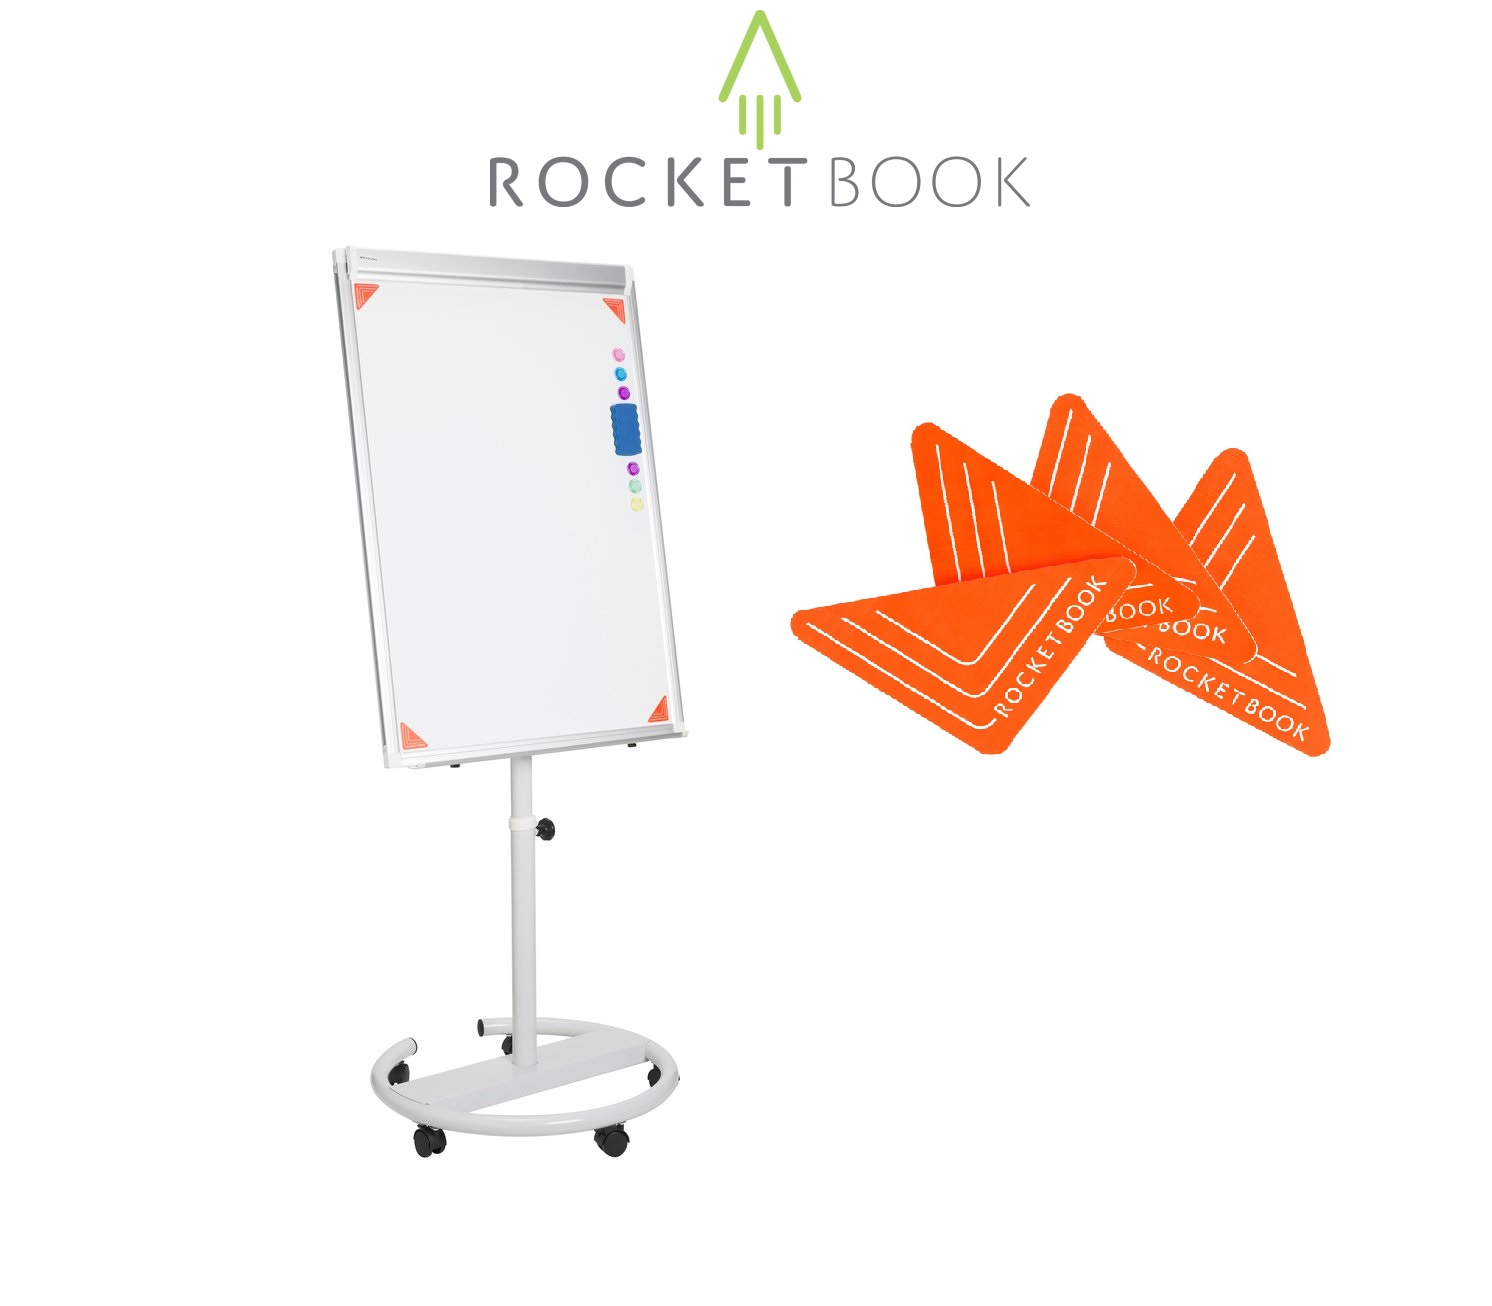
\includegraphics[width=1\linewidth]{becons.png}
	\caption{Rocketbook Beacons \cite{Rocketbook}}
	\label{fig:ROCK}
\end{figure}

\begin{figure}
	\centering
	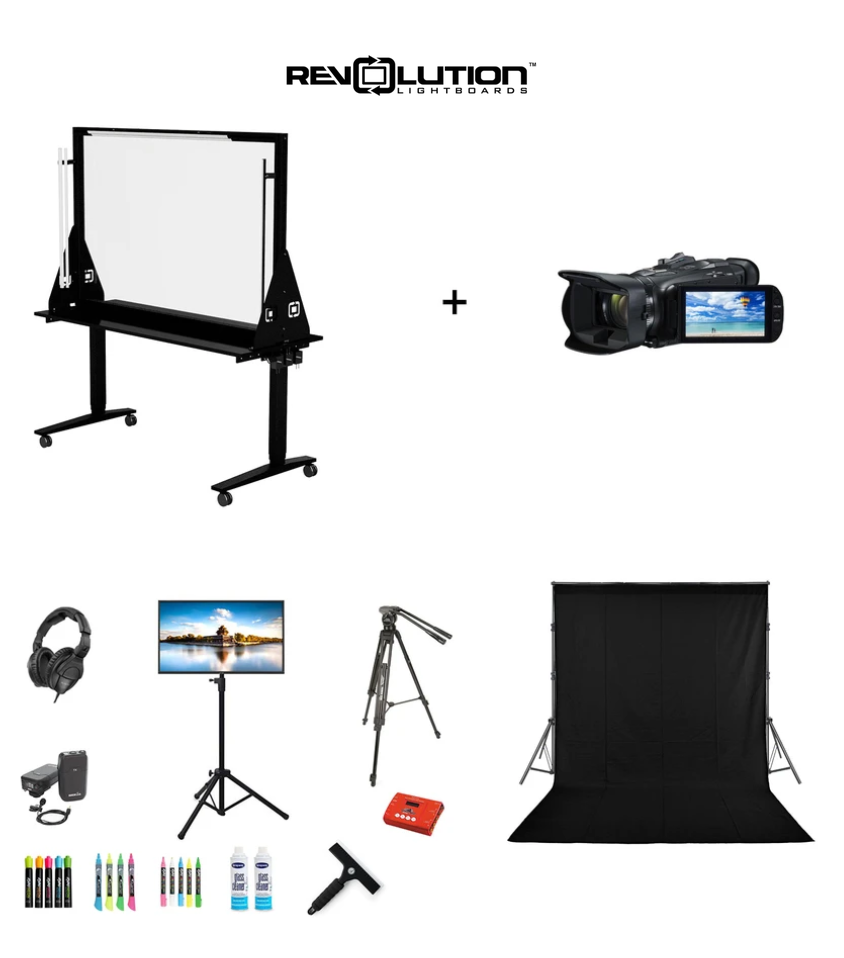
\includegraphics[width=1\linewidth]{Revolution.png}
	\caption{ Studio Package from Revolution Lightboards \cite{Revolution}}
	\label{fig:REV}
\end{figure}






\section{Design}
%What was the process used to develop the chosen design and implement it? Remember to cite if using existing methodology!
Axiomatic design is implemented in our design, they are only rules (axiom) that needs to follow\cite{suh2001axiomatic}.  
\begin{quote}
	Axiom 1, the independence axiom:
	Maintain the independence of the functional requirements
	
	Axiom 2, the information axiom:
	Minimize the information content of the design
\end{quote}

%Assumptions stated (there are always some)
We assume that there will be 230V mains where electric power is needed and users have a room where no sunlight is and the walls are dark (darkroom).     % ??????fleira SENTI JOE EMAIL???????

%Design DP0, DP1-7.  First a Noun; can be quanitified or compared.
\subsection{Physical Solution}\label{PS}
The Physical solution for the Functional requirement in chapter \ref{FR} are;
\begin{quote} 
	\textbf{\PS0} : Lightboard with mechanical linkage system.
\end{quote}

\begin{quote} 
	\textbf{\PS1} : Linkage bar system for camera. \\ 
	\textbf{Metric :} Length between camera and lightboard is $2 m \pm 0.05 m$ and height is $1.5 m$.
\end{quote}

\begin{quote} 
	\textbf{\PS2} : Linkage bar system for lights.
	\\ \textbf{Metric :} Bar is 45° out from the lightboard.
\end{quote}

\begin{quote} 
	\textbf{\PS3} : Linkage bar system for mic.
	\\ \textbf{Metric :} Mic is pointing to the mouth of the teacher when he stands in the middle of lightboard.
\end{quote}

\begin{quote} 
	\textbf{\PS4} : Hinges on linkage system.
	\\ \textbf{Metric :} Hinges rotate min 135°.
\end{quote}

\begin{quote} 
	\textbf{\PS5} : Wheel under the frame.
	\\ \textbf{Metric :} Loading min 500 N per wheel and castor wheels.
\end{quote}

%Design matrix and discussion of coupling: uncoupled, decoupled, coupled
The Design Decomposition flowchart is shown in figure \ref{fig:matrix}.
This system is decoupled (path-dependent) because $FR_1$, $FR_2$ and $FR_3$ need to have two physical solutions to fulfill the functional requirement.
In other words, how camera, light, and mic are guided to its place depends on the hinges.
A decoupled design is worse than an uncoupled but still allows the exact adjustment of the functional requirements.\cite{system_design}.


%Detailed explanation of how each DP was implemented
\textbf{\PS1} Is implemented with a linkage system from the lightboard.
Two hinges make it foldable.
When folded it is in the correct height and length from the lightboard.
The length was estimated after a trip to a lightboard studio setup with StudyHax.

\textbf{\PS2} The same linkage system design is used for the three lights.
Hinges are used for the foldability of the arms and give the desired angle of the lights.
The length is 700 mm that gives the lights the proper distance from the lightboard after measuring the distance in StudyHax studio.

\textbf{\PS3} The linkage system that is used for the light above the teacher is used here.
Because of the x-profile, it is possible to put a holder on the side of the linkage system that holds the mic in place.
The holder can be placed in different angles in the right direction.

\textbf{\PS4} Next to the lightboard for the lights will be a hinge (see B in figure \ref{fig:Finalprodotype2} ) that can move the linkage system in desired angle.
For the camera will be two hinges to fold the camera stand.

\textbf{\PS5} Under the frame is 4 castor wheels with the brake as is shown in C in figure \ref{fig:Finalprodotype2}.
They will be fixed with bolts and nuts to the frame.

%Modular Dependency Diagram or System Diagram
Modular Dependency Diagram or System Diagram can be seen in figure \ref{fig:scematic}
\begin{figure}
	\centering
	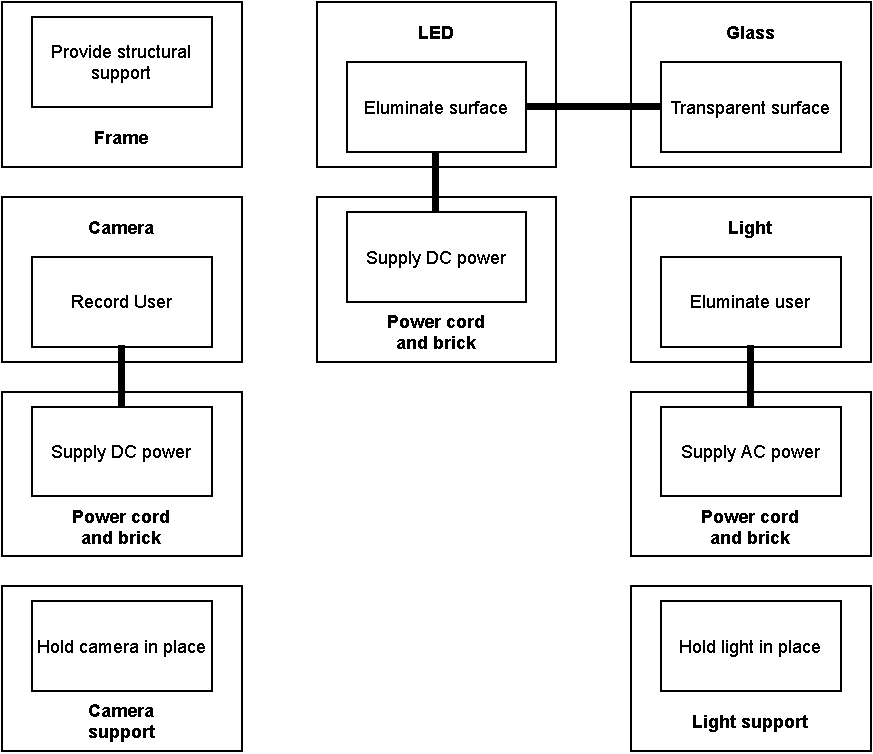
\includegraphics[width=1\linewidth]{scematic.pdf}
	\caption{The schematic of Lightboard Ready}
	\label{fig:scematic}
\end{figure}


%CAD Drawing (circuit schematic or other)
\begin{figure}
	\centering
	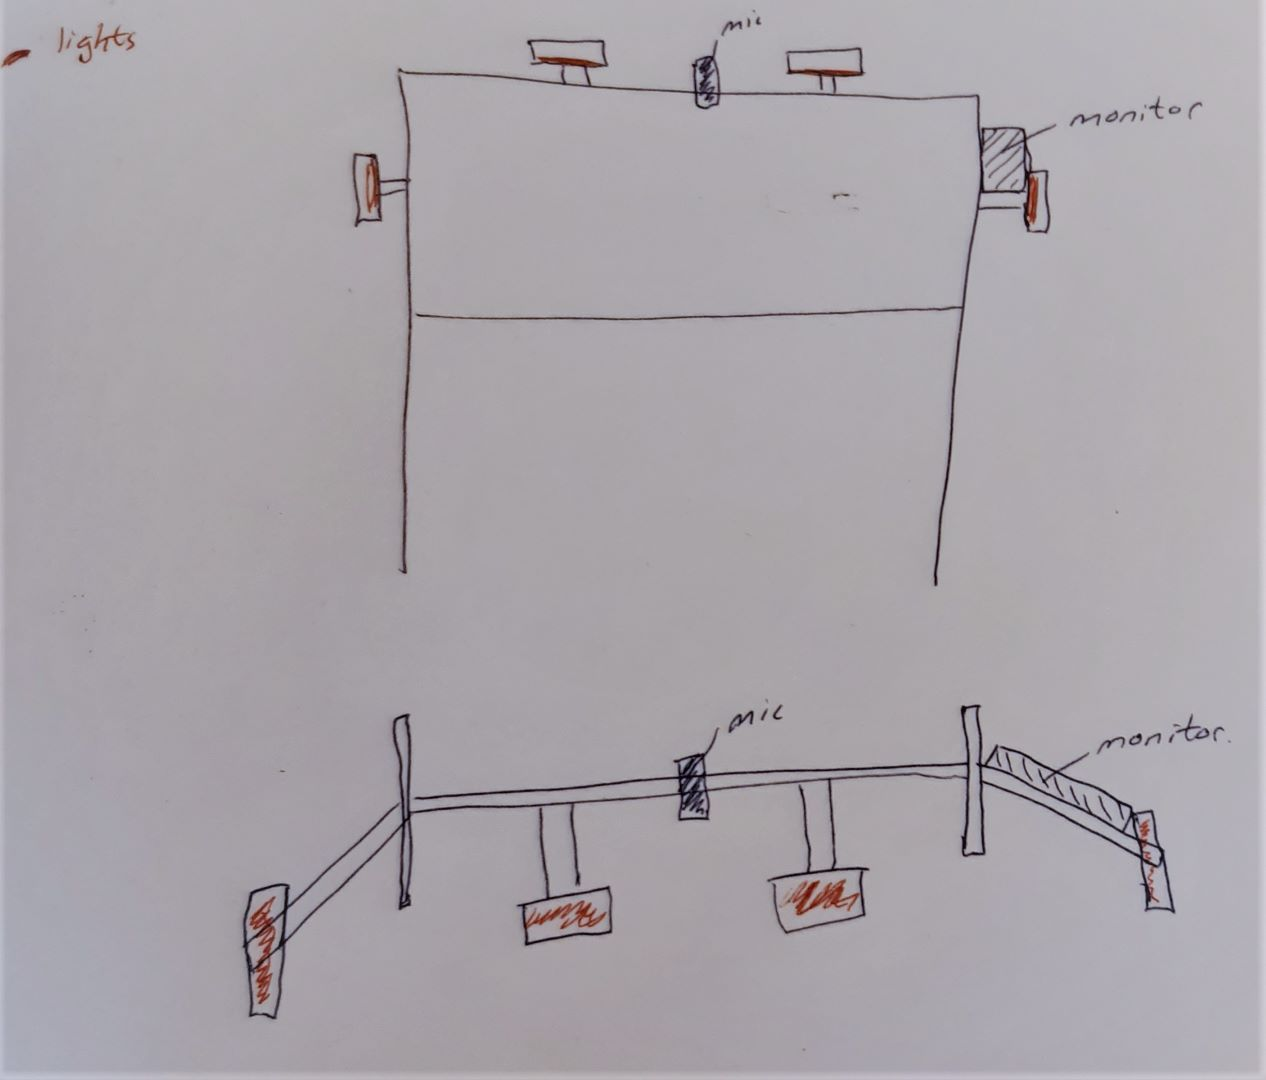
\includegraphics[width=1\linewidth]{skissa_1.jpg}
	\caption{Sketches of different concepts}\label{fig:Sketchesofdifferentconcepts}
\end{figure}
\begin{figure}
	\centering
	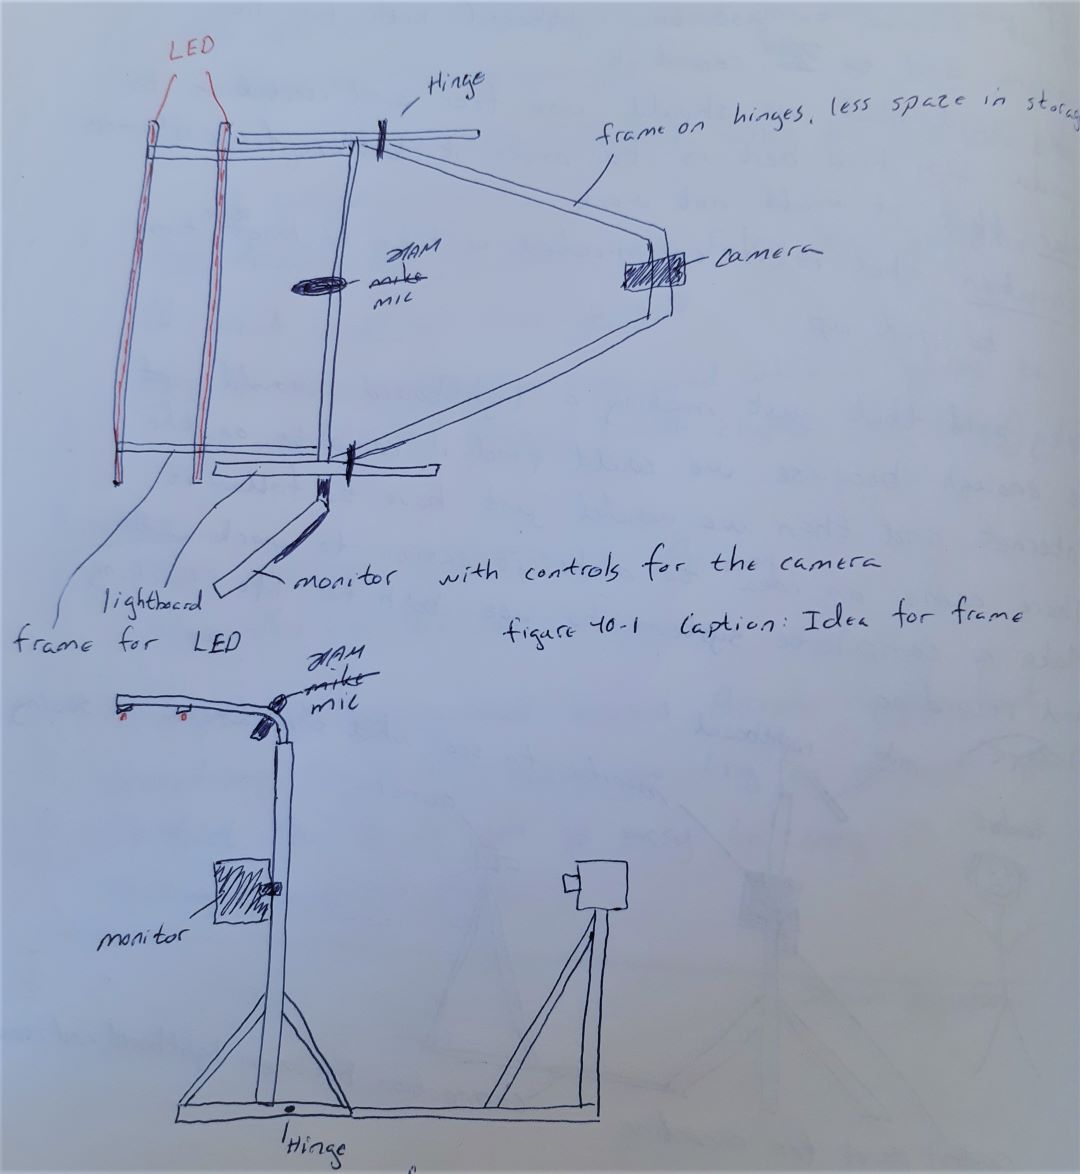
\includegraphics[width=1\linewidth]{skissa_2.jpg}
	\caption{Sketches of different concepts}\label{fig:Sketchesofdifferentconcepts2}
\end{figure}

\begin{figure}
	\centering
	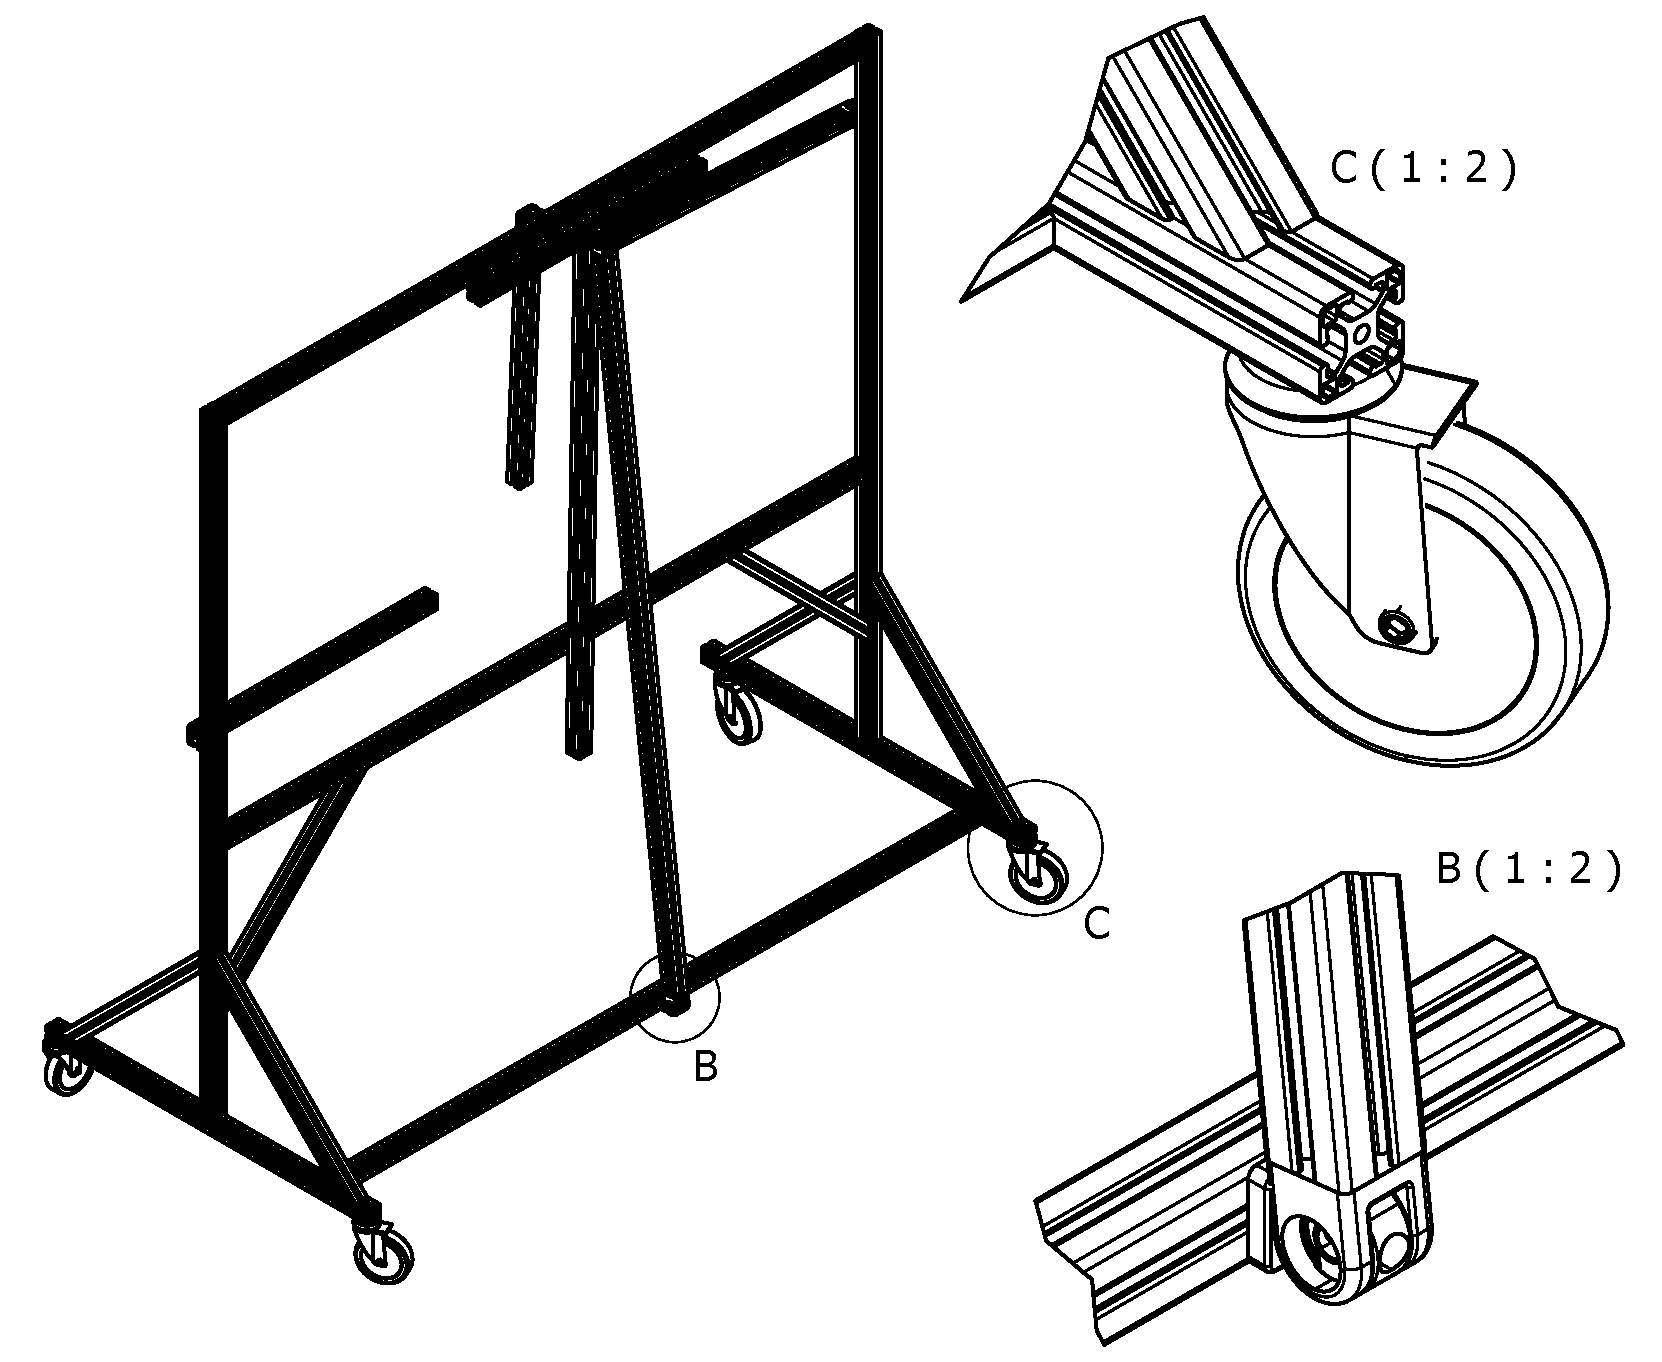
\includegraphics[width=1\linewidth]{frame2.pdf}
	\caption{Lightboard ready folded with detail view of the hinge and caster that is used}
	\label{fig:Finalprodotype2}
\end{figure}






%Stages of design and refinement to show the progression from idea to finished system
Figure \ref{fig:Sketchesofdifferentconcepts} shows our first idea of the concept.  It shows a sketch of a linkage system connected to a lightboard.
There are lights on the sides and lights above the teacher.
Also is a v-shaped linkage system for the camera.
Figure \ref{fig:pappi_1} and \ref{fig:pappi_3} shows a physical model of the idea but there we have added hinges on the linkage system for the light so the system would take less space in storage.
The beta prototype is shown in figure \ref{fig:Finalprodotype} and shows the lightboard built with x-profiles and the linkage system for the lights and mic has hinges for foldability.
The linkage system for the camera has been simplified and this structure makes the feet on the lightboard more robust. There is a latent need with this design, that is it's possible to move the camera stand closer to the writing surface if needed.
There are hinges on the camera linkage that goes away from the lightboard so it has foldability, and also a beam with rubber dampers on the camera stand that makes the camera stand stable.
Under the frame are castor wheels with brakes for mobility.

%Pictures of the final prototype
The final prototype can be seen in figure \ref{fig:Finalprodotype}.

\section{Results and Discussion}
%This is a subjective section. Is there data and discussion here? Explain challenges that would be of interest to a reader and how you solved them. Remember that the reader does not care if you found the exercise “interesting” or “learned a lot”. Instead, they would like to know what things are of interest to someone in this field of research. What things should they learn? What problems arose and how did you solve them? Be specific and detailed. You should also justify your statements with data. This is a good place to put analysis (including equations) and simulation.


%What needed to be tested and why?
The 
%How did you setup your tests?  (details on setup and execution)
%Quantitative data from tests?
%Power consumption (Watts)
%Mass of system
%What does the data mean?
%Discussion of the system's performance

\subsection{Testing the concept}

%How are you going to test it?  Make a plan.
This idea is going to be tested with building the frame for the camera stand and mount it to a lightboard that we have access to.
For the lights, we will make an adjustable arm to hold them in the correct position and also mount them on the lightboard.
In figure \ref{fig:pappi_1} is a physical model that shows the layout of the lightboard with lights and camera stand ready for use.
In figure \ref{fig:pappi_3} is it folded together for transport or storage.\\
The plan for the test is to have a dark room that we can put up our equipment for recording a short video that shows how this idea works.
The video is going to show both what is seen in videos made with this and also the layout of our equipment.

\begin{figure}
	\centering 
	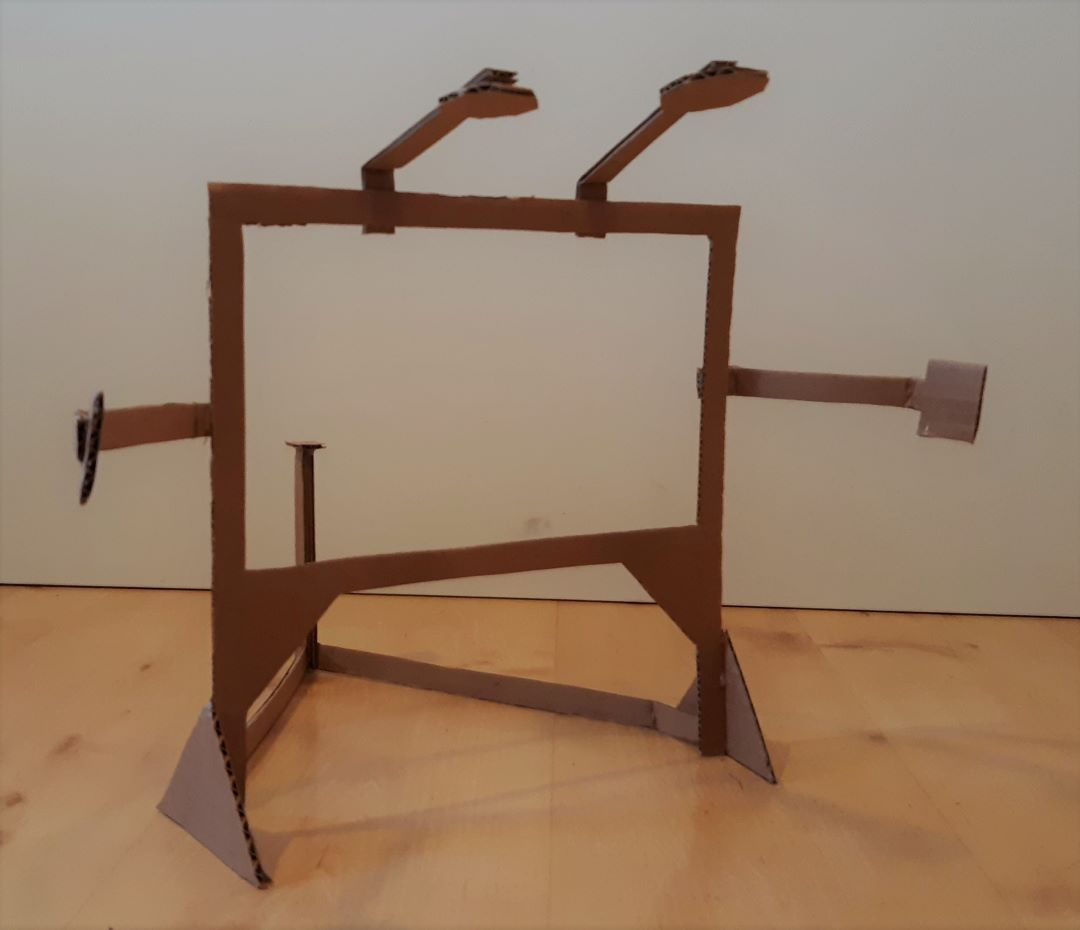
\includegraphics[width=1\linewidth]{pappi_1.jpg}
	\caption{Physical model}
	\label{fig:pappi_1}
\end{figure}
\begin{figure}
	\centering
	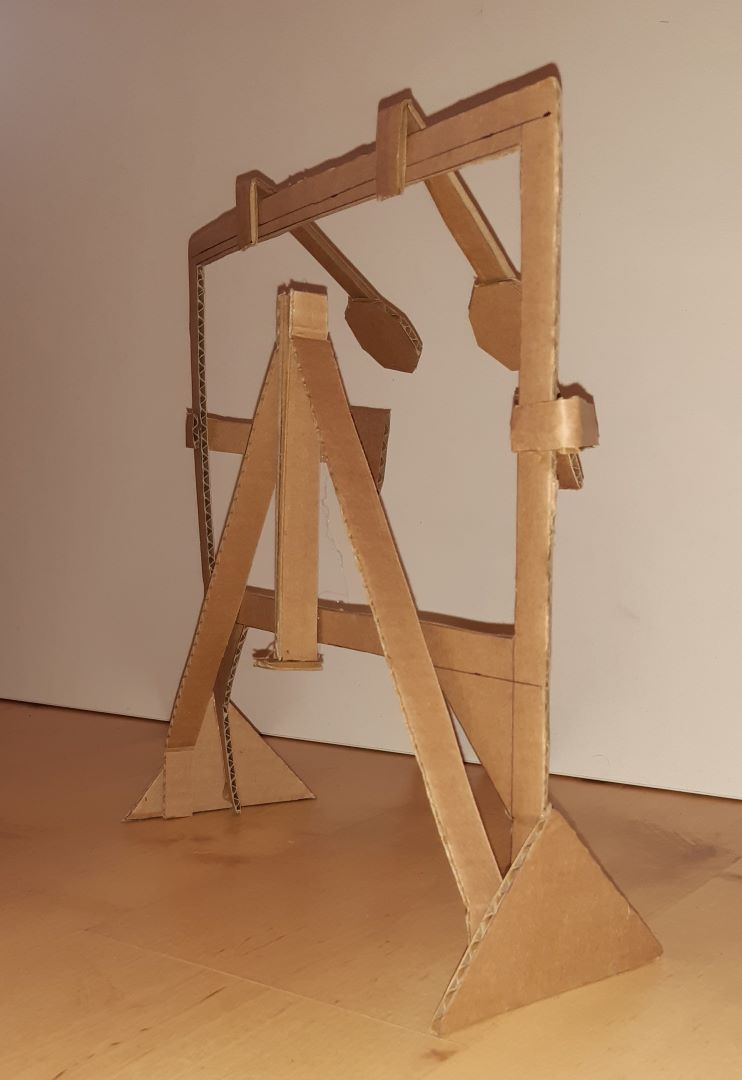
\includegraphics[width=1\linewidth]{pappi_3.jpg}
	\caption{Physical model, folded together}
	\label{fig:pappi_3}
\end{figure}
\section{Product Architecture}
The product line is two, Medium (2m width ) and Large (3m width ). Both of them have a 16:9 ratio so the camera and video will cover the whole glass without it need to stretch or crop the recordings.
One possible assignment of elements to chunks is shown in figure \ref{fig:scematic}.
The importance of industrial design in the development of the Lightboard Ready are shown in table \ref{tab:importnace}





%\section{ Importance of industrial design}
\begin{table}
	\centering
		\begin{tabular}{lll}
			\textbf{Ergonomics}& Level of importance & Explanation\\
			\hline
			Ease of use  & 
			\setlength{\fboxsep}{0pt}\fbox{\IosSevenSlider{2.5cm}{1}} & 
			So people with  little light and camera settings  \\ &&  experience canuse lightbord. \\
			Ease of maintenance  &
			\setlength{\fboxsep}{0pt} \fbox{\IosSevenSlider{2.5cm}{0.1}} & 
			The system is robust with little mobility\\
			Quantity of interaction &\setlength{\fboxsep}{0pt}\fbox{\IosSevenSlider{2.5cm}{0.3}}  & 
			There are only two function onthe product, assemble  \\ &&  and disassemble .\\
			Novelty of user interaction &
			\setlength{\fboxsep}{0pt}\fbox{\IosSevenSlider{2.5cm}{0.8}}  &
			The product is  known, but not  with this installation. \\
			Safety & \setlength{\fboxsep}{0pt}\fbox{\IosSevenSlider{2.5cm}{0.9}}  & 
			There are  safety  issues because  it is possible to get\\ && stuck between two rods. \\
			\hline
			\textbf{Aesthetics} & 
			&\\
			Product differential & 
			\setlength{\fboxsep}{0pt}
			\fbox{\IosSevenSlider{2.5cm}{0.1}} & 
			This is a new method\\
			Pride of ownership &
			\setlength{\fboxsep}{0pt}
			\fbox{\IosSevenSlider{2.5cm}{0.1}} &
			It is a matter of \\ &&comfort.\\
			Team motivation & 
			\setlength{\fboxsep}{0pt}
			\fbox{\IosSevenSlider{2.5cm}{0.5}} &
			It is a new concept
			
		\end{tabular}
	\caption{Assessing the importance of industrial design for  Lightboard Ready}
	\label{tab:importnace}
\end{table}
\section{Design for Manufacturing}


% 1. Detailed Bill of Materials

\begin{figure*}
	\centering
	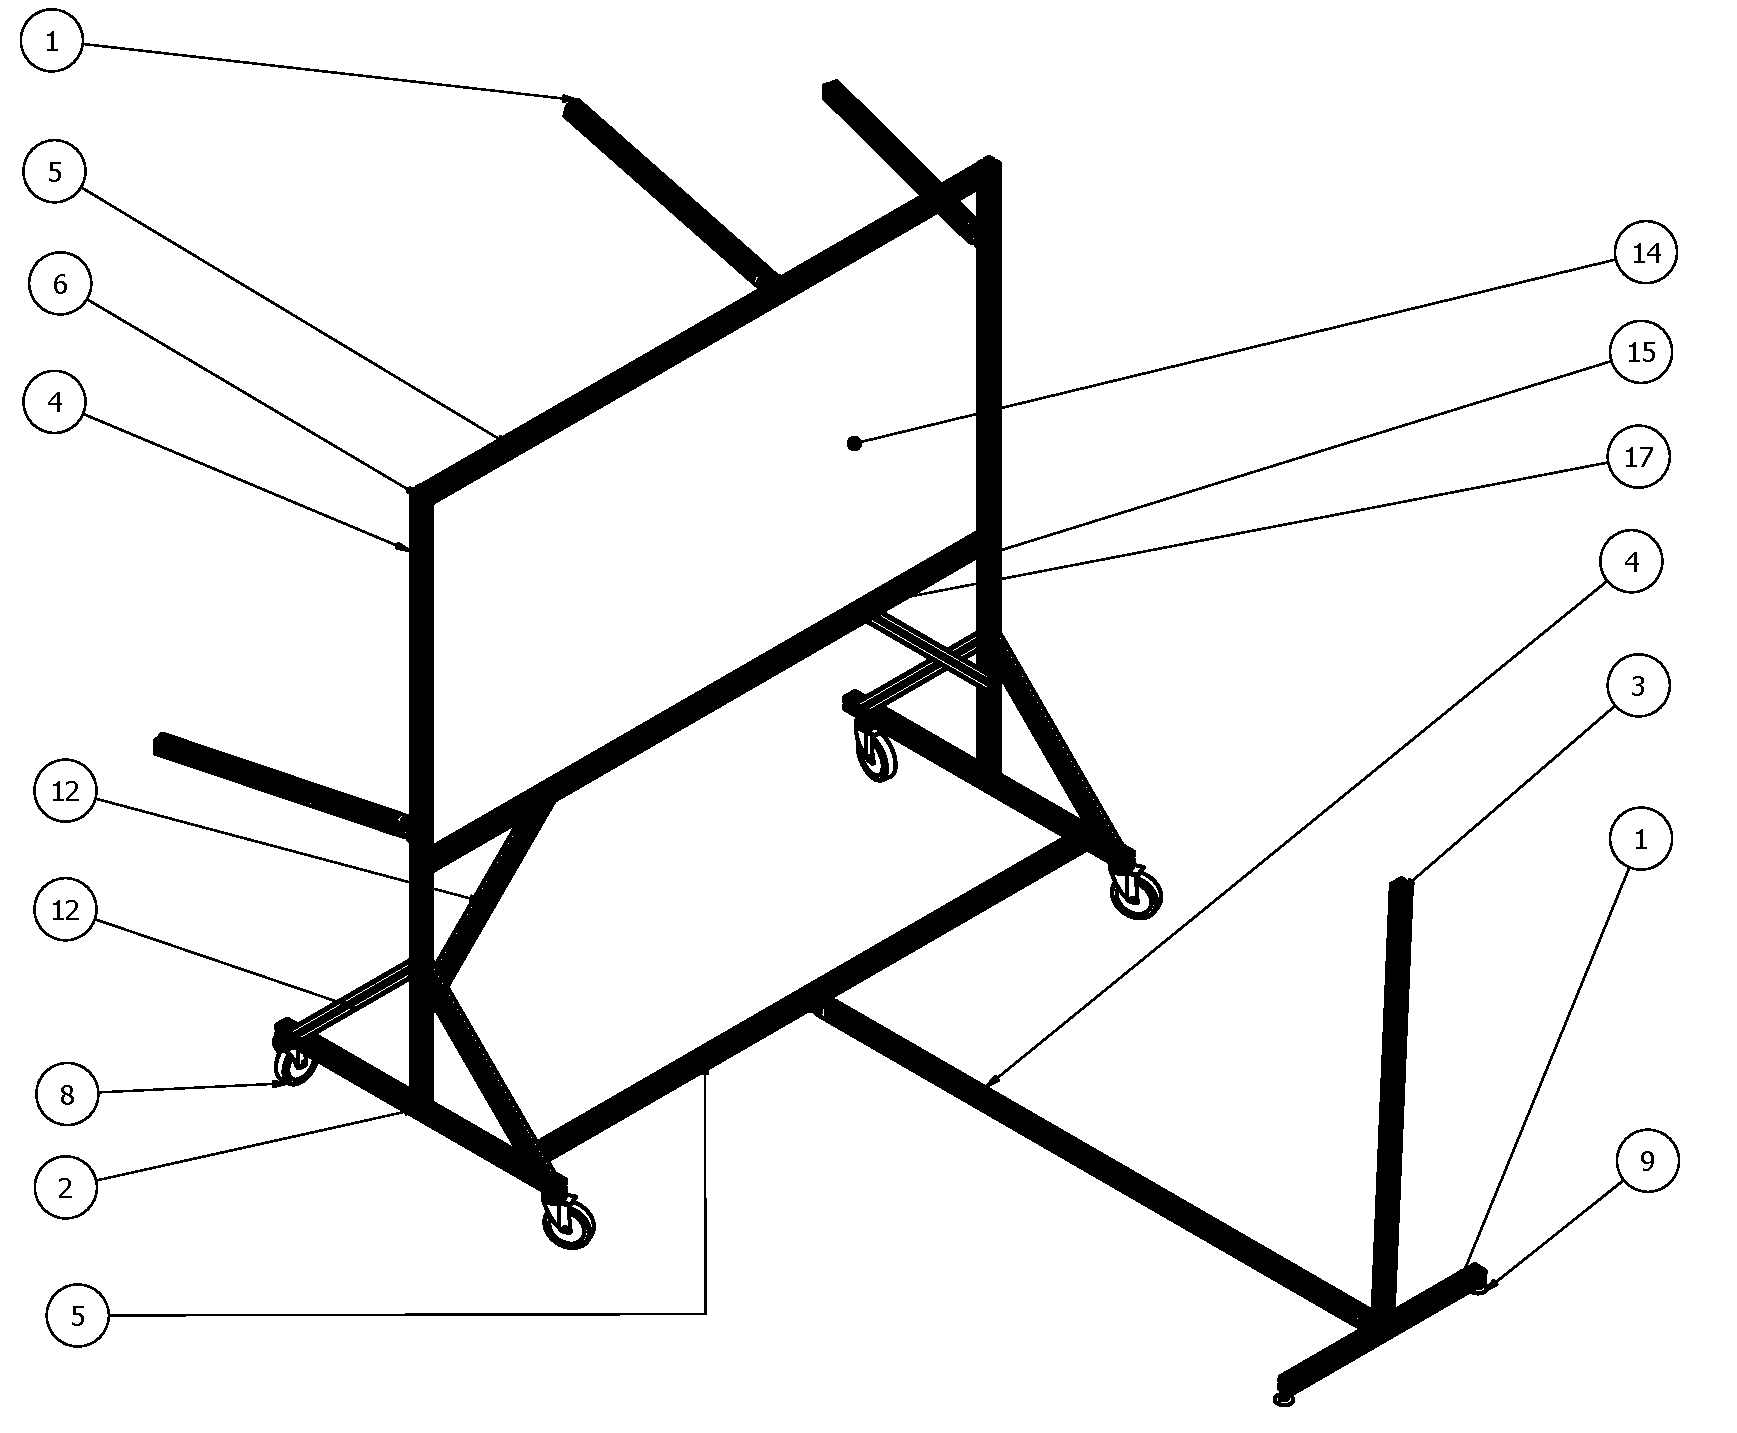
\includegraphics[width=1\linewidth]{frame1.pdf}
	\caption{Lightboard ready}
	\label{fig:Finalprodotype}
\end{figure*}

\begin{table*}[]
	\centering
	\begin{tabular}{llrrr}
		
		Part nr. & Component & Material & Number of parts  \\
		\hline
		1&4040-Lite-Black 700mm  & Aluminium  & 4  \\
		2&4040-Lite-Black 1000mm & Aluminium &  2\\
		3&4040-Lite-Black 1400mm & Aluminium & 1  \\
		4&4040-Lite-Black 1900mm & Aluminium & 3  \\
		5&4040-Lite-Black 2000mm  & Aluminium &3  \\
		6&Standard Anchor Fastener  & Galvanic steel&4  \\
		7&Double Anchor Fastener  &Galvanic steel & 4  \\
		8&Caster with brake  & Galvanic steel and rubber & 4  \\
		9&Floor Nylon-Glide  & Nylon& 2 \\
		10&2 Hole-Pivot Joint  & Galvanic steel & 5  \\
		11&Self-Aligning T-Nut  & Galvanic steel &4   \\
		12&45 Degree Support 640mm  & Aluminium &  6 \\
		13&45 Degree Support 160mm  & Aluminium & 2  \\
		14&Starphire Glass& Glass &1\\
		15&LED Strip& & 1\\
		16&Power Supply & & 1 \\
		17&Black Glass Gasket & Thermoplastic Elastomer & 1\\
		18&Packaging & Cardboard & 1  \\ %\hline
	\end{tabular}
	\caption{Bill of material }
	\label{tab:BOM}
\end{table*}


% 2. The estimated cost of manufacturing your product for the quantities you expect to sell
The market in Iceland is schools at all levels.% and companies that could see this as a way to teach new employees the basics in videos.
There are 237 schools in Iceland\cite{skolar}.
So we estimate that every third school will buy and then the market for Lightboard Ready is 80 units.
%The market is also the whole world but then it would be done with partners to safe transport.
%The market is also the whole world with internet sale.
\begin{table*}[]
	\centering
	\begin{tabular}{lrr|r}
		\hline
		Component & \multicolumn{1}{l}{\begin{tabular}[c]{@{}l@{}}Purchased \\ Materials\end{tabular}} &  \multicolumn{1}{l|}{\begin{tabular}[c]{@{}l@{}}Assembly \\ (Labor)\end{tabular}} & \multicolumn{1}{l}{\begin{tabular}[c]{@{}l@{}}Total Unit\\ Variable\\ Cost\end{tabular}} \\ \hline
		4040-Lite-Black 700mm  & 53.79 &  & 53.79 \\
		4040-Lite-Black 1000mm  & 49.56 &  & 49.56 \\
		4040-Lite-Black 1400mm & 33.92 & \textbf{} & 33.92 \\
		4040-Lite-Black 1900mm  & 143.82 &  & 143.82 \\
		4040-Lite-Black 2000mm  & 158.46 &  & 158.46 \\
		Standard Anchor Fastener  & 14.80  &  & 14.80 \\
		Double Anchor Fastener  & 23.20  &  & 23.20 \\
		Caster with brake  & 41.20 &   & 41.20 \\
		Floor Nylon-Glide  & 4.80  &  & 4.80 \\
		2 Hole-Pivot Joint  & 94.50  &  & 94.50 \\
		Self-Aligning T-Nut  & 7.20  &  & 7.20 \\
		45 Degree Support 640mm  & 198.90  &  & 198.90 \\
		45 Degree Support 160mm  & 35.80  &  & 35.80 \\
		Black Glass Gasket & 12.25 & & 12.25\\
		Starphire Glass & 264.00 & & 264.00 \\
		LED Strip & 29.99 & & 29.99 \\
		Power Supply & 26.50 & & 26.50\\
		Packaging & 5.00 & 20.00 & 25.00 \\ \hline
		Total Direct Costs & 1197.69.89 & 20.00 & 1217.69 \\
		Overhead Charges & 119.8  & 5 & 125.58 \\
		Transport from Supplier & & & 97.66 \\
		\textbf{Total Cost} &   &  & \textbf{1440.93} \\ \hline
	\end{tabular}
	\caption{Cost estimate in USD \cite{8020} \cite{ispan}}
	\label{tab:cost}
\end{table*}

We are buying everything in correct lengths and drilled so there is no labor cost in table \ref{tab:cost} except for the packaging.
These prices are found on 80/20.net and then the transport cost is estimated from that all 80 units are imported in one container.
The reason that USD is used is that the ISK is always changing and on the BOM list is everything imported except for the glass. 

% 3. Answer:  How are you reducing the cost of components, assembly, and supporting production?
Lightboard Ready is going to be sold dissembled  %like IKEA does it, 
in flat boxes and the buyer %puts itself together.
assemble it themself and 
this will % save assembly cost but it also makes the size of the packaging lot smaller, transportation easier and %the transport cost is less.
thereby making it cheaper.
This design uses only two angles in cutting, 90 and 45 degrees.
All combinations on the x-profile fit together so it is possible to use standard connections that are cheaper.
It also makes this design for the frame more robust.
\section{Design for Environment}
% Answer how you are doing these things in your product or why you cannot


%1.Design products and processes with industrial materials that can be recycled continually with no loss in performance, thereby creating new industrial materials.
Lightboard Ready is made mostly out of Aluminium, galvanic steel and glass wish can be recycled constantly without loss of performance and thereby create new industrial material.
%2.Design products and processes with natural materials that can be fully returned to the earth’s natural cycles, thereby creating new natural materials.
The only natural material in Lightboard ready is the packaging, wish is a cardboard that fully recycles or can fully return to earth natural cycles, and thereby create new natural material.

%3.Design products and processes that do not produce unnatural, toxic materials that cannot be safely processed by either natural or industrial cycles.
No toxin material cannot be safely processed by either natural or industrial cycles.

%4.Design products and processes with clean, renewable sources of energy, rather than fossil fuels.
The product is assembled in Iceland that has renewable and clean energy.
The glass is made in Iceland with renewable energy.
The x-profiles are coming from a supplier that uses aluminum produced in Iceland in their product. 


\section{Experiments}

\section{Results and Discussion}

\section{Conclusion}

\subsection{Future work}

\subsection{Summary}

\section*{References}
\bibliography{iopart-num-demo,references,references-ad}

\end{document}



%%% Local Variables:
%%% mode: latex
%%% TeX-master: t
%%% End:
